%%
%% Beginning of file 'paper.tex'
%%
%% Modified 2018 January
%%
%% This is a sample manuscript marked up using the
%% AASTeX v6.2 LaTeX 2e macros.
%%
%% AASTeX is now based on Alexey Vikhlinin's emulateapj.cls 
%% (Copyright 2000-2015).  See the classfile for details.

%% AASTeX requires revtex4-1.cls (http://publish.aps.org/revtex4/) and
%% other external packages (latexsym, graphicx, amssymb, longtable, and epsf).
%% All of these external packages should already be present in the modern TeX 
%% distributions.  If not they can also be obtained at www.ctan.org.

%% The first piece of markup in an AASTeX v6.x document is the \documentclass
%% command. LaTeX will ignore any data that comes before this command. The 
%% documentclass can take an optional argument to modify the output style.
%% The command below calls the preprint style  which will produce a tightly 
%% typeset, one-column, single-spaced document.  It is the default and thus
%% does not need to be explicitly stated.
%%
%%
%% using aastex version 6.2
\documentclass{aastex62}

%% The default is a single spaced, 10 point font, single spaced article.
%% There are 5 other style options available via an optional argument. They
%% can be envoked like this:
%%
%% \documentclass[argument]{aastex62}
%% 
%% where the layout options are:
%%
%%  twocolumn   : two text columns, 10 point font, single spaced article.
%%                This is the most compact and represent the final published
%%                derived PDF copy of the accepted manuscript from the publisher
%%  manuscript  : one text column, 12 point font, double spaced article.
%%  preprint    : one text column, 12 point font, single spaced article.  
%%  preprint2   : two text columns, 12 point font, single spaced article.
%%  modern      : a stylish, single text column, 12 point font, article with
%% 		  wider left and right margins. This uses the Daniel
%% 		  Foreman-Mackey and David Hogg design.
%%  RNAAS       : Preferred style for Research Notes which are by design 
%%                lacking an abstract and brief. DO NOT use \begin{abstract}
%%                and \end{abstract} with this style.
%%
%% Note that you can submit to the AAS Journals in any of these 6 styles.
%%
%% There are other optional arguments one can envoke to allow other stylistic
%% actions. The available options are:
%%
%%  astrosymb    : Loads Astrosymb font and define \astrocommands. 
%%  tighten      : Makes baselineskip slightly smaller, only works with 
%%                 the twocolumn substyle.
%%  times        : uses times font instead of the default
%%  linenumbers  : turn on lineno package.
%%  trackchanges : required to see the revision mark up and print its output
%%  longauthor   : Do not use the more compressed footnote style (default) for 
%%                 the author/collaboration/affiliations. Instead print all
%%                 affiliation information after each name. Creates a much
%%                 long author list but may be desirable for short author papers
%%
%% these can be used in any combination, e.g.
%%
%% \documentclass[twocolumn,linenumbers,trackchanges]{aastex62}
%%
%% AASTeX v6.* now includes \hyperref support. While we have built in specific
%% defaults into the classfile you can manually override them with the
%% \hypersetup command. For example,
%%
%%\hypersetup{linkcolor=red,citecolor=green,filecolor=cyan,urlcolor=magenta}
%%
%% will change the color of the internal links to red, the links to the
%% bibliography to green, the file links to cyan, and the external links to
%% magenta. Additional information on \hyperref options can be found here:
%% https://www.tug.org/applications/hyperref/manual.html#x1-40003
%%
%% If you want to create your own macros, you can do so
%% using \newcommand. Your macros should appear before
%% the \begin{document} command.
%%
\newcommand{\vdag}{(v)^\dagger}
\newcommand\aastex{AAS\TeX}
\newcommand\latex{La\TeX}

%% Tells LaTeX to search for image files in the 
%% current directory as well as in the figures/ folder.
\graphicspath{{./}{figures/}}

%% Reintroduced the \received and \accepted commands from AASTeX v5.2
\received{January 1, 2018}
\revised{January 7, 2018}
\accepted{\today}
%% Command to document which AAS Journal the manuscript was submitted to.
%% Adds "Submitted to " the arguement.
\submitjournal{ApJ}

%% Mark up commands to limit the number of authors on the front page.
%% Note that in AASTeX v6.2 a \collaboration call (see below) counts as
%% an author in this case.
%
%\AuthorCollaborationLimit=3
%
%% Will only show Schwarz, Muench and "the AAS Journals Data Scientist 
%% collaboration" on the front page of this example manuscript.
%%
%% Note that all of the author will be shown in the published article.
%% This feature is meant to be used prior to acceptance to make the
%% front end of a long author article more manageable. Please do not use
%% this functionality for manuscripts with less than 20 authors. Conversely,
%% please do use this when the number of authors exceeds 40.
%%
%% Use \allauthors at the manuscript end to show the full author list.
%% This command should only be used with \AuthorCollaborationLimit is used.

%% The following command can be used to set the latex table counters.  It
%% is needed in this document because it uses a mix of latex tabular and
%% AASTeX deluxetables.  In general it should not be needed.
%\setcounter{table}{1}

%%%%%%%%%%%%%%%%%%%%%%%%%%%%%%%%%%%%%%%%%%%%%%%%%%%%%%%%%%%%%%%%%%%%%%%%%%%%%%%%
%%
%% The following section outlines numerous optional output that
%% can be displayed in the front matter or as running meta-data.
%%
%% If you wish, you may supply running head information, although
%% this information may be modified by the editorial offices.
%%
%% You can add a light gray and diagonal water-mark to the first page 
%% with this command:
% \watermark{text}
%% where "text", e.g. DRAFT, is the text to appear.  If the text is 
%% long you can control the water-mark size with:
%  \setwatermarkfontsize{dimension}
%% where dimension is any recognized LaTeX dimension, e.g. pt, in, etc.
%%
%%%%%%%%%%%%%%%%%%%%%%%%%%%%%%%%%%%%%%%%%%%%%%%%%%%%%%%%%%%%%%%%%%%%%%%%%%%%%%%%

%% This is the end of the preamble.  Indicate the beginning of the
%% manuscript itself with \begin{document}.
\usepackage{listings}
\usepackage{minted}
\begin{document}

\title{EinsteinPy: Python for General Relativity\footnote{Released on July, 15th, 2019}}

%% LaTeX will automatically break titles if they run longer than
%% one line. However, you may use \\ to force a line break if
%% you desire. In v6.2 you can include a footnote in the title.

%% A significant change from earlier AASTEX versions is in the structure for 
%% calling author and affilations. The change was necessary to implement 
%% autoindexing of affilations which prior was a manual process that could 
%% easily be tedious in large author manuscripts.
%%
%% The \author command is the same as before except it now takes an optional
%% arguement which is the 16 digit ORCID. The syntax is:
%% \author[xxxx-xxxx-xxxx-xxxx]{Author Name}
%%
%% This will hyperlink the author name to the author's ORCID page. Note that
%% during compilation, LaTeX will do some limited checking of the format of
%% the ID to make sure it is valid.
%%
%% Use \affiliation for affiliation information. The old \affil is now aliased
%% to \affiliation. AASTeX v6.2 will automatically index these in the header.
%% When a duplicate is found its index will be the same as its previous entry.
%%
%% Note that \altaffilmark and \altaffiltext have been removed and thus 
%% can not be used to document secondary affiliations. If they are used latex
%% will issue a specific error message and quit. Please use multiple 
%% \affiliation calls for to document more than one affiliation.
%%
%% The new \altaffiliation can be used to indicate some secondary information
%% such as fellowships. This command produces a non-numeric footnote that is
%% set away from the numeric \affiliation footnotes.  NOTE that if an
%% \altaffiliation command is used it must come BEFORE the \affiliation call,
%% right after the \author command, in order to place the footnotes in
%% the proper location.
%%
%% Use \email to set provide email addresses. Each \email will appear on its
%% own line so you can put multiple email address in one \email call. A new
%% \correspondingauthor command is available in V6.2 to identify the
%% corresponding author of the manuscript. It is the author's responsibility
%% to make sure this name is also in the author list.
%%
%% While authors can be grouped inside the same \author and \affiliation
%% commands it is better to have a single author for each. This allows for
%% one to exploit all the new benefits and should make book-keeping easier.
%%
%% If done correctly the peer review system will be able to
%% automatically put the author and affiliation information from the manuscript
%% and save the corresponding author the trouble of entering it by hand.

\author[0000-0002-0870-4665]{Shreyas Bapat}
\affiliation{School of Computing and Electrical Engineering, Indian Institute of Technology Mandi, India}

\author{Bhavya Bhatt}
\affiliation{School of Computing and Electrical Engineering, Indian Institute of Technology Mandi, India}

\author{Ritwik Saha}
\affiliation{School of Computing and Electrical Engineering, Indian Institute of Technology Mandi, India}

\author[0000-0003-1021-3336]{Priyanshu Khandelwal}
\affiliation{School of Computing and Electrical Engineering, Indian Institute of Technology Mandi, India}
\collaboration{(EinsteinPy Core Development Committee)}

\author[0000-0002-2268-9772]{Sofía Ortín Vela}
\affil{Department of Theoretical Physics, University of Zaragoza, Spain}

\author[0000-0001-8530-7252]{Jialin Ma}
\affil{Georgia Institute of Technology, USA}

\author[0000-0001-7234-6148]{Varun Singh}
\affiliation{School of Computing and Electrical Engineering, Indian Institute of Technology Mandi, India}

\author[0000-0002-1900-3338]{Shilpi Jain}
\affiliation{Department of Earth Sciences, Indian Institute of Technology Roorkee, India}

\author[0000-0002-7179-3795]{Alpesh Jamgade}
\affiliation{Department of Mathematics, Bharath Institute of Higher Education and Research, Chennai, India}

\author[0000-0002-5198-9010]{Manvi Gupta}
\affiliation{School of Computing and Electrical Engineering, Indian Institute of Technology Mandi, India}

\author{Tushar Tyagi}
\affiliation{School of Computing and Electrical Engineering, Indian Institute of Technology Mandi, India}

\author[0000-0003-1838-8368]{Tanmay Rustagi}
\affiliation{School of Computing and Electrical Engineering, Indian Institute of Technology Mandi, India}

\author[0000-0002-0757-2883]{Abhijeet Manhas}
\affiliation{School of Computing and Electrical Engineering, Indian Institute of Technology Mandi, India}

\author[0000-0001-5558-9447]{Raphael Reyna}
\affiliation{California State Polytechnic University, Pomona}

\author[0000-0001-8302-1584]{Sashank Mishra}
\affiliation{Department of Information Technology, Indian Institute of Information Technology Allahabad}
\collaboration{(EinsteinPy Package Contributors)}
%% Note that the \and command from previous versions of AASTeX is now
%% depreciated in this version as it is no longer necessary. AASTeX 
%% automatically takes care of all commas and "and"s between authors names.

%% AASTeX 6.2 has the new \collaboration and \nocollaboration commands to
%% provide the collaboration status of a group of authors. These commands 
%% can be used either before or after the list of corresponding authors. The
%% argument for \collaboration is the collaboration identifier. Authors are
%% encouraged to surround collaboration identifiers with ()s. The 
%% \nocollaboration command takes no argument and exists to indicate that
%% the nearby authors are not part of surrounding collaborations.

%% Mark off the abstract in the ``abstract'' environment. 
\begin{abstract}

This paper presents EinsteinPy (version 0.2), a community-developed Python
package for gravitational and relativistic astrophysics. Python is a free, easy to use high level programming language which has seen a huge expansion in the number of its users and developers in recent years. Specifically, a lot of recent studies show that the use of Python in Astrophysics and in general physics has increased exponentially. Many great frameworks came as Python packages which provide a very high level of abstraction over the dirty nitty-gritty of complex algorithms and provide an easy to use interfaceand pleasing user experience. One such example is Keras - framework for deep learning which has made deep learning so easy that a person with zero programming knowledge can also train a neural network classifier. This example really demonstrates the power of abstraction which is achievable in Python. The aim of the EinsteinPy is no different and is developed keeping in mind the state of a theoretical gravitational physicist with a little or no background in computer programming and trying to work in the field of numerical relativity or trying to use simulations in their research. Currently EinsteinPy supports simulation of time-like and null geodesics and calculate trajectories in different background geometries some of which are Schwarzschild, Kerr and KerrNewmann along with coordinate inter-conversion pipeline. It has a partially developed pipeline for plotting and visualization with dependencies on libraries like plotly, matplotlib etc. One of the unique feature of EinsteinPy is a sufficiently developed symbolic tensor manipulation utilites which is a great tool in itself for teaching yourself tensor algebra which for many beginner students can be overwhelmingly tricky. Currently EinsteinPy also provide few utility functions for hypersurface embedding of Schwarzschild spacetime which further will be extended to model gravitational lensing simulation. The current version of the library is in a state that can be used by any serious student of general relativity trying to get essence of this beautiful subject but is somewhere lost in the heavy mathematical formalism of the subject. EinsteinPy provides such students to really see through the equations and visualize whats really happening.


\end{abstract}

%% Keywords should appear after the \end{abstract} command. 
%% See the online documentation for the full list of available subject
%% keywords and the rules for their use.
\keywords{gravitational physics, astrophysics --- 
simulations --- black holes --- gravitational waves}

%% From the front matter, we move on to the body of the paper.
%% Sections are demarcated by \section and \subsection, respectively.
%% Observe the use of the LaTeX \label
%% command after the \subsection to give a symbolic KEY to the
%% subsection for cross-referencing in a \ref command.
%% You can use LaTeX's \ref and \label commands to keep track of
%% cross-references to sections, equations, tables, and figures.
%% That way, if you change the order of any elements, LaTeX will
%% automatically renumber them.
%%
%% We recommend that authors also use the natbib \citep
%% and \citet commands to identify citations.  The citations are
%% tied to the reference list via symbolic KEYs. The KEY corresponds
%% to the KEY in the \bibitem in the reference list below. 

\section{Introduction} \label{sec:intro}
It was the time of 1915 when Einstein published his paper on general theory of relativity which proposed a elegant and rigorous framework for a relativistic theory of gravity and was generalized version of gravity free theory - special relativity which he published earlier in 1905 and since then the whole physics community was against the bold ideas of the young genius and resisted in the beginning because all people were worried that if these hypothesis true would then completely change our notion of how we percieve space and time. But sooner they started to realize the true depth in the formalism of general relativity and its ability to explain the fundamental laws of nature. After so many years its well established now that general theory of relativity is the "theory of gravity" in classical regime and all the attempts to formulate quantum theory of gravity one way or the other borrow ideas from GR. The central problem then and now remains to be the solutions of the Einstein's field equation. Many times we can study the behaviour of solutions under high degree of symmetry considerations and could even solve analytically for highly unrealistic systems but solving it for problems relevant to astrophysical and gravitational physics research it still remains a big question on how to get around the problem of solving these field equations. This question is so profound that it has a separate research field which goes with the name of numerical relativity which attempts to use computer programmes to numerically obtain solutions of the equations (which would be the background geometry) for some turbulent region where most of the interesting dynamics is happening (as we can not solve for a infinitely large grid due to restrictions imposed on us by space and time complexity and computability).\\
The interest of the community grew when the field found applications in areas of radio astronomy, cosmology, signal processing, data mining. After so many years the field of numerical relativity has grown up to be a mature research area with vast literature on algorithms, numerical methods and theoretical formulations (from basic 3+1 decomposition formulation to more sophisticated ones). Currently there exist some very robust and involved frameworks that provide a complete programming ecosystem and have proved to an be essential tools for any numerical relativity researcher. Now on the other end of the research community are the theoretical physicists many of which have little or no programming experience and is really challenged by the fact that the usage of these frameworks demand heavy use of high level programming languages like C and C++. As described above Python provides a vast room for abstractions and no library existed at that time that do numerical relativity in Python and hence the team was hooked by this very fact of need for a python library on general relativity. Since then EinsteinPy has seen a lot of contributions from people all over the world and many "good to go" functionalities are already provided in this and previous versions. Like any other numerical relativity library EinsteinPy is made to provide a set of tools which can make numerical computations for solving Einstein's field equations an easy job for anyone who does not want to dive deep into the nitty gitties of the subject along with few very basic but powerful functionalities that could be used by anyone who wants to learn the subject of general relativity in general\footnote{More details on this are given in further coming sections}. In further coming section we discuss with some of the features of the current as well previous version and the future plans which are yet to be implemented in the upcoming versions. Also we describe few code snippets to explain the usage of the library on which more details can be found on the organisation website\footnote{https://einsteinpy.org/}
\section{Units Handling}
EinsteinPy has dependencies on Astropy for handling units and user have to use appropiate Astropy units\footnote{more on astropy units can be refered from their official website documentation} while declaring the input data to various methods which are further used in computation. 
\section{Data Types} \label{sec:style}
The heart of abstraction that EinsteinPy aims to provide is achieved by some set of data structures that are specifically designed to ease with variety of gravitational physics problems. The most important and central quantity in all of the general relativity is the metric tensor $g_{\mu\nu}$ which defines the background geometry of spacetime on which all the dynamics happen. Informally the problem that packages of numerical relativity tend to solve is that we have a system (or matter field) defined by energy-momentum tensor $T_{\mu\nu}$ and we want to solve for the $g_{\mu\nu}$ such that it satifies the following Einstein's field equation
\[
R_{\mu\nu} - \frac{1}{2}Rg_{\mu\nu} + \Lambda g_{\mu\nu} = \frac{8\pi G}{c^4}T_{\mu\nu}
\]where $R_{\mu\nu}$ is contracted Riemannian tensor or Ricci tensor, $R$ is Ricci scalar, $\Lambda$ is cosmological constant. All the above quantities are derivatives of metric tensor\footnote{more on this can be refered from any standard general relativity text} so in simple terms, on the left hand side of the equation are terms involving $g_{\mu\nu}$ and on the right hand side are the matter field terms which only characterize the distribution of matter.\\
EinsteinPy provides a core module: \texttt{metric} which has core data types of various metric tensors some which includes Schwarzschild, Kerr, Kerr-Newman spacetime geometries(which are exact solution of field equation for very specific matter distributions). The immediate functionalities which comes along with this module is solution of geodesic equations. The module has coupled integration with \texttt{coordinates} module which deals with different coordinate system transformations\footnote{more on this in the 'coordinates' section}. Another core data types is in the \texttt{plotting} module which handles all the plotting, rendering, animation and simulation related methods and provides a user friendly interfacing of plots. One interesting feature of EinsteinPy is the support for symbolic tensor algebra which is extremly important in the formalism of general relativity and one of the first challenges faced by many beginners in their journey of learning the subject. EinsteinPy provides an excellent way to learn the math behind tensor manipulation and index gymnastics with the help of symbolic module: \texttt{symbolic}, on which more will be dicussed in its section ahead.\\
Following sections will give a breif overview of every core module and some of their important functionalities.
\subsection{tensor}
\subsection{metric}
\texttt{metric} module give users the freedom to define metric object which can be further used in the computations related to spacetime geometry. Let's see an small example of solving geodesic equation in Kerr spacetime and obtaining trajectories using EinsteinPy
\subsection{coordinates}
\begin{minted}[linenos]{python}
# importing modules
from astropy import units as u
import numpy as np
from einsteinpy.metric import Kerr
from einsteinpy.coordinates import BoyerLindquistDifferential

# initializing parameters and coordinate system
M = 1.989e30 * u.kg
a = 0.3 * u.m
BL_obj = BoyerLindquistDifferential(50e5 * u.km, np.pi / 2 * u.rad, np.pi * u.rad,
                                    0 * u.km / u.s, 0 * u.rad / u.s, 0 * u.rad / u.s,
                                    a)
end_lambda = ((1 * u.year).to(u.s)).value / 930

# Choosing stepsize for ODE solver to be 0.02 minutes
stepsize = ((0.02 * u.min).to(u.s)).value

# defining Kerr spacetime metric object
obj = Kerr.from_coords(BL_obj, M)

# calculates the trajectory
ans = obj.calculate_trajectory(
    end_lambda=end_lambda, OdeMethodKwargs={"stepsize": stepsize}, return_cartesian=True
)
\end{minted}
\subsection{plotting}
\subsection{symbolic}
\subsection{hypersurface}
This module provides with basic computational functions which are essential for modelling the space-like hypersurface for any spacetime geometry. Currently module has implementation for Schwarzschild geometry with conversion functions from Schwarzschild coordinates to 3-D spherical coordinates and some plotting utilities. The whole module is expected to extend for providing a superclass for implementations related to gravitationl lensing simulations and numerical calculations of null geodesics on hypersurfaces and deviation angles for systems which are relevant to relativistic astrophysical problems. A small code snippet for plotting the hypersurface is as follows:
\begin{minted}[linenos]{python}
# importing the modules
from einsteinpy.hypersurface import SchwarzschildEmbedding
from astropy import units as u

# Declaring embedding object with specified mass of the body 
surface_obj = SchwarzschildEmbedding(5.927e23 * u.kg)
surface_obj.plot_hypersurface(plot_type='surface')

# plotting the embedding hypersurface for Schwarzschild spacetime
surface_obj.show()
\end{minted}
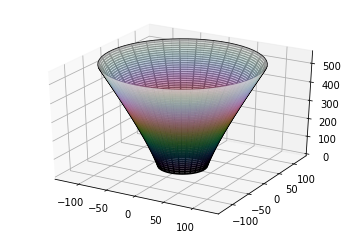
\includegraphics[scale=0.5]{hypersurface_surface.png}
 
\section{Displaying mathematics} \label{sec:displaymath}

The most common mathematical symbols and formulas are in the amsmath
package.  \aastex\ requires this package so there is no need to
specifically call for it in the document preamble.  Most modern \latex\
distributions already contain this package.  If you do not have this
package or the other required packages, revtex4-1, latexsym, graphicx,
amssymb, longtable, and epsf, they can be obtained from 
\url{http://www.ctan.org}

Mathematics can be displayed either within the text, e.g. $E = mc^2$, or
separate from in an equation.  In order to be properly rendered, all inline
math text has to be declared by surrounding the math by dollar signs (\$).

A complex equation example with inline math as part of the explanation
follows.

\begin{equation}
\bar v(p_2,\sigma_2)P_{-\tau}\hat a_1\hat a_2\cdots
\hat a_nu(p_1,\sigma_1) ,
\end{equation}
where $p$ and $\sigma$ label the initial $e^{\pm}$ four-momenta
and helicities $(\sigma = \pm 1)$, $\hat a_i=a^\mu_i\gamma_\nu$
and $P_\tau=\frac{1}{2}(1+\tau\gamma_5)$ is a chirality projection
operator $(\tau = \pm1)$.  This produces a single line formula.  \latex\ will
auto-number this and any subsequent equations.  If no number is desired then
the {\tt\string equation} call should be replaced with {\tt\string displaymath}.

\latex\ can also handle a a multi-line equation.  Use {\tt\string eqnarray}
for more than one line and end each line with a
\textbackslash\textbackslash.  Each line will be numbered unless the
\textbackslash\textbackslash\ is preceded by a {\tt\string\nonumber}
command.  Alignment points can be added with ampersands (\&).  There should be
two ampersands per line. In the examples they are centered on the equal
symbol.

\begin{eqnarray}
\gamma^\mu  & = &
 \left(
\begin{array}{cc}
0 & \sigma^\mu_+ \\
\sigma^\mu_- & 0
\end{array}     \right) ,
 \gamma^5= \left(
\begin{array}{cc}
-1 &   0\\
0 &   1
\end{array}     \right)  , \\
\sigma^\mu_{\pm}  & = &   ({\bf 1} ,\pm \sigma) , 
\end{eqnarray}

\begin{eqnarray}
\hat a & = & \left(
\begin{array}{cc}
0 & (\hat a)_+\\
(\hat a)_- & 0
\end{array}\right), \nonumber \\
(\hat a)_\pm & = & a_\mu\sigma^\mu_\pm 
\end{eqnarray}

%% Putting eqnarrays or equations inside the mathletters environment groups
%% the enclosed equations by letter. For instance, the eqnarray below, instead
%% of being numbered, say, (4) and (5), would be numbered (4a) and (4b).
%% LaTeX the paper and look at the output to see the results.

\section{Revision tracking and color highlighting} \label{sec:highlight}

Authors sometimes use color to highlight changes to their manuscript in
response to editor and referee comments.  In \aastex\ new commands
have been introduced to make this easier and formalize the process. 

The first method is through a new set of editing mark up commands that
specifically identify what has been changed.  These commands are
{\tt\string\added\{<text>\}}, {\tt\string\deleted\{<text>\}}, and
{\tt\string\replaced\{<old text>\}\{<replaced text>\}}. To activate these
commands the {\tt\string trackchanges} option must be used in the
{\tt\string\documentclass} call.  When compiled this will produce the
marked text in red.  The {\tt\string\explain\{<text>\}} can be used to add
text to provide information to the reader describing the change.  Its
output is purple italic font. To see how {\tt\string\added\{<important
added info>\}}, {\tt\string\deleted\{<this can be deleted text>\}},
{\tt\string\replaced\{<old data>\}\{<replaced data>\}}, and \break
{\tt\string\explain\{<text explaining the change>\}} commands will produce
\added{important added information}\deleted{, deleted text, and }
\replaced{old data}{and replaced data,} toggle between versions compiled with
and without the {\tt\string trackchanges} option.\explain{text explaining
the change}

A summary list of all these tracking commands can be produced at the end of
the article by adding the {\tt\string\listofchanges} just before the
{\tt\string\end\{document\}} call.  The page number for each change will be
provided. If the {\tt\string linenumbers} option is also included in the
documentcall call then not only will all the lines in the article be
numbered for handy reference but the summary list will also include the
line number for each change.

The second method does not have the ability to highlight the specific
nature of the changes but does allow the author to document changes over
multiple revisions.  The commands are {\tt\string\edit1\{<text>\}},
{\tt\string\edit2\{<text>\}} and {\tt\string\edit3\{<text>\}} and they
produce {\tt\string<text>} that is highlighted in bold red, italic blue and
underlined purple, respectively.  Authors should use the first command to
\edit1{indicated which text has been changed from the first revision.}  The
second command is to highlight \edit2{new or modified text from a second
revision}.  If a third revision is needed then the last command should be used 
\edit3{to show this changed text}.  Since over 90\% of all manuscripts are
accepted after the 3rd revision these commands make it easy to identify
what text has been added and when.  Once the article is accepted all the
highlight color can be turned off simply by adding the
{\tt\string\turnoffediting} command in the preamble. Likewise, the new commands
{\tt\string\turnoffeditone}, {\tt\string\turnoffedittwo}, and
{\tt\string\turnoffeditthree} can be used to only turn off the 
{\tt\string\edit1\{<text>\}}, {\tt\string\edit2\{<text>\}} and 
{\tt\string\edit3\{<text>\}}, respectively.

Similar to marking editing changes with the {\tt\string\edit} options there
are also the {\tt\string\authorcomments1\{<text>\}}, 
{\tt\string\authorcomments2\{<text>\}} and
{\tt\string\authorcomments3\{<text>\}} commands.  These produce the same
bold red, italic blue and underlined purple text but when the
{\tt\string\turnoffediting} command is present the {\tt\string<text>}
material does not appear in the manuscript.  Authors can use these commands
to mark up text that they are not sure should appear in the final
manuscript or as a way to communicate comments between co-authors when
writing the article.

\section{Software and third party data repository citations} \label{sec:cite}

The AAS Journals would like to encourage authors to change software and
third party data repository references from the current standard of a
footnote to a first class citation in the bibliography.  As a bibliographic
citation these important references will be more easily captured and credit
will be given to the appropriate people.

The first step to making this happen is to have the data or software in
a long term repository that has made these items available via a persistent
identifier like a Digital Object Identifier (DOI).  A list of repositories
that satisfy this criteria plus each one's pros and cons are given at \break
\url{https://github.com/AASJournals/Tutorials/tree/master/Repositories}.

In the bibliography the format for data or code follows this format: \\

\noindent author year, title, version, publisher, prefix:identifier\\

\citet{2015ApJ...805...23C} provides a example of how the citation in the
article references the external code at
\doi{10.5281/zenodo.15991}.  Unfortunately, bibtex does
not have specific bibtex entries for these types of references so the
``@misc'' type should be used.  The Repository tutorial explains how to
code the ``@misc'' type correctly.  The most recent aasjournal.bst file,
available with \aastex\ v6, will output bibtex ``@misc'' type properly.

%% If you wish to include an acknowledgments section in your paper,
%% separate it off from the body of the text using the \acknowledgments
%% command.
\acknowledgments

We thank all the people that have made this AASTeX what it is today.  This
includes but not limited to Bob Hanisch, Chris Biemesderfer, Lee Brotzman,
Pierre Landau, Arthur Ogawa, Maxim Markevitch, Alexey Vikhlinin and Amy
Hendrickson. Also special thanks to David Hogg and Daniel Foreman-Mackey
for the new "modern" style design. Considerable help was provided via bug
reports and hacks from numerous people including Patricio Cubillos, Alex
Drlica-Wagner, Sean Lake, Michele Bannister, Peter Williams, and Jonathan
Gagne.

%% To help institutions obtain information on the effectiveness of their 
%% telescopes the AAS Journals has created a group of keywords for telescope 
%% facilities.
%
%% Following the acknowledgments section, use the following syntax and the
%% \facility{} or \facilities{} macros to list the keywords of facilities used 
%% in the research for the paper.  Each keyword is check against the master 
%% list during copy editing.  Individual instruments can be provided in 
%% parentheses, after the keyword, but they are not verified.

\vspace{5mm}
\facilities{HST(STIS), Swift(XRT and UVOT), AAVSO, CTIO:1.3m,
CTIO:1.5m,CXO}

%% Similar to \facility{}, there is the optional \software command to allow 
%% authors a place to specify which programs were used during the creation of 
%% the manusscript. Authors should list each code and include either a
%% citation or url to the code inside ()s when available.

\software{astropy \citep{2013A&A...558A..33A},  
          Cloudy \citep{2013RMxAA..49..137F}, 
          SExtractor \citep{1996A&AS..117..393B}
          }

%% Appendix material should be preceded with a single \appendix command.
%% There should be a \section command for each appendix. Mark appendix
%% subsections with the same markup you use in the main body of the paper.

%% Each Appendix (indicated with \section) will be lettered A, B, C, etc.
%% The equation counter will reset when it encounters the \appendix
%% command and will number appendix equations (A1), (A2), etc. The
%% Figure and Table counter will not reset.

\appendix

\section{Appendix information}

Appendices can be broken into separate sections just like in the main text.
The only difference is that each appendix section is indexed by a letter
(A, B, C, etc.) instead of a number.  Likewise numbered equations have
the section letter appended.  Here is an equation as an example.

\begin{equation}
I = \frac{1}{1 + d_{1}^{P (1 + d_{2} )}}
\end{equation}

Appendix tables and figures should not be numbered like equations. Instead
they should continue the sequence from the main article body.

\section{Author publication charges} \label{sec:pubcharge}

Finally some information about the AAS Journal's publication charges.
In April 2011 the traditional way of calculating author charges based on 
the number of printed pages was changed.  The reason for the change
was due to a recognition of the growing number of article items that could not 
be represented in print. Now author charges are determined by a number of
digital ``quanta''.  A single quantum is 350 words, one figure, one table,
and one enhanced digital item.  For the latter this includes machine readable
tables, figure sets, animations, and interactive figures.  The current cost
is \$27 per word quantum and \$30 for all other quantum type.

\section{Rotating tables} \label{sec:rotate}

The process of rotating tables into landscape mode is slightly different in
\aastex v6.2. Instead of the {\tt\string\rotate} command, a new environment
has been created to handle this task. To place a single page table in a
landscape mode start the table portion with
{\tt\string\begin\{rotatetable\}} and end with
{\tt\string\end\{rotatetable\}}.

Tables that exceed a print page take a slightly different environment since
both rotation and long table printing are required. In these cases start
with {\tt\string\begin\{longrotatetable\}} and end with
{\tt\string\end\{longrotatetable\}}. Table \ref{chartable} is an
example of a multi-page, rotated table.

\begin{longrotatetable}
\begin{deluxetable*}{lllrrrrrrll}
\tablecaption{Observable Characteristics of 
Galactic/Magellanic Cloud novae with X-ray observations\label{chartable}}
\tablewidth{700pt}
\tabletypesize{\scriptsize}
\tablehead{
\colhead{Name} & \colhead{V$_{max}$} & 
\colhead{Date} & \colhead{t$_2$} & 
\colhead{FWHM} & \colhead{E(B-V)} & 
\colhead{N$_H$} & \colhead{Period} & 
\colhead{D} & \colhead{Dust?} & \colhead{RN?} \\ 
\colhead{} & \colhead{(mag)} & \colhead{(JD)} & \colhead{(d)} & 
\colhead{(km s$^{-1}$)} & \colhead{(mag)} & \colhead{(cm$^{-2}$)} &
\colhead{(d)} & \colhead{(kpc)} & \colhead{} & \colhead{}
} 
\startdata
CI Aql & 8.83 (1) & 2451665.5 (1) & 32 (2) & 2300 (3) & 0.8$\pm0.2$ (4) & 1.2e+22 & 0.62 (4) & 6.25$\pm5$ (4) & N & Y \\
{\bf CSS081007} & \nodata & 2454596.5 & \nodata & \nodata & 0.146 & 1.1e+21 & 1.77 (5) & 4.45$\pm1.95$ (6) & \nodata & \nodata \\
GQ Mus & 7.2 (7) & 2445352.5 (7) & 18 (7) & 1000 (8) & 0.45 (9) & 3.8e+21  & 0.059375 (10) & 4.8$\pm1$ (9) & N (7) & \nodata \\
IM Nor & 7.84 (11) & 2452289 (2) & 50 (2) & 1150 (12) & 0.8$\pm0.2$ (4) & 8e+21 & 0.102 (13) & 4.25$\pm3.4$ (4) & N & Y \\
{\bf KT Eri} & 5.42 (14) & 2455150.17 (14) & 6.6 (14) & 3000 (15) & 0.08 (15) & 5.5e+20 & \nodata & 6.5 (15) & N & M \\
{\bf LMC 1995} & 10.7 (16) & 2449778.5 (16) & 15$\pm2$ (17) & \nodata & 0.15 (203) & 7.8e+20  & \nodata & 50 & \nodata & \nodata \\
LMC 2000 & 11.45 (18) & 2451737.5 (18) & 9$\pm2$ (19) & 1700 (20) & 0.15 (203) & 7.8e+20  & \nodata & 50 & \nodata & \nodata \\
{\bf LMC 2005} & 11.5 (21) & 2453700.5 (21) & 63 (22) & 900 (23) & 0.15 (203) & 1e+21 & \nodata & 50  & M (24) & \nodata \\
{\bf LMC 2009a} & 10.6 (25) & 2454867.5 (25) & 4$\pm1$  & 3900 (25) & 0.15 (203)  & 5.7e+20 & 1.19 (26) & 50 & N & Y \\
{\bf SMC 2005} & 10.4 (27) & 2453588.5 (27) & \nodata & 3200 (28) & \nodata & 5e+20  & \nodata & 61 & \nodata & \nodata \\
{\bf QY Mus} & 8.1 (29) & 2454739.90 (29) & 60:  & \nodata & 0.71 (30) & 4.2e+21  & \nodata & \nodata & M & \nodata \\
{\bf RS Oph} & 4.5 (31) & 2453779.44 (14) & 7.9 (14) & 3930 (31) & 0.73 (32) & 2.25e+21 & 456 (33) & 1.6$\pm0.3$ (33) & N (34) & Y \\
{\bf U Sco} & 8.05 (35) & 2455224.94 (35) & 1.2 (36) & 7600 (37) & 0.2$\pm0.1$ (4) & 1.2e+21 & 1.23056 (36) & 12$\pm2$ (4) & N & Y \\
{\bf V1047 Cen} & 8.5 (38) & 2453614.5 (39) & 6 (40) & 840 (38) & \nodata & 1.4e+22  & \nodata & \nodata & \nodata & \nodata \\
{\bf V1065 Cen} & 8.2 (41) & 2454123.5 (41) & 11 (42) & 2700 (43) & 0.5$\pm0.1$ (42) & 3.75e+21 & \nodata & 9.05$\pm2.8$ (42) & Y (42) & \nodata \\
V1187 Sco & 7.4 (44) & 2453220.5 (44) & 7: (45) & 3000 (44) & 1.56 (44) & 8.0e+21 & \nodata & 4.9$\pm0.5$ (44) & N & \nodata \\
{\bf V1188 Sco} & 8.7 (46) & 2453577.5 (46) & 7 (40) & 1730 (47) & \nodata & 5.0e+21  & \nodata & 7.5 (39) & \nodata & \nodata \\
{\bf V1213 Cen} & 8.53 (48) & 2454959.5 (48) & 11$\pm2$ (49) & 2300 (50) & 2.07 (30) & 1.0e+22 & \nodata & \nodata & \nodata & \nodata \\
{\bf V1280 Sco} & 3.79 (51) & 2454147.65 (14) & 21 (52) & 640 (53) & 0.36 (54) & 1.6e+21  & \nodata & 1.6$\pm0.4$ (54) & Y (54) & \nodata \\
{\bf V1281 Sco} & 8.8 (55) & 2454152.21 (55) & 15:& 1800 (56) & 0.7 (57) & 3.2e+21 & \nodata & \nodata & N & \nodata \\
{\bf V1309 Sco} & 7.1 (58) & 2454714.5 (58) & 23$\pm2$ (59) & 670 (60) & 1.2 (30) & 4.0e+21 & \nodata & \nodata & \nodata & \nodata \\
{\bf V1494 Aql} & 3.8 (61) & 2451515.5 (61) & 6.6$\pm0.5$ (61) & 1200 (62) & 0.6 (63) & 3.6e+21  & 0.13467 (64) & 1.6$\pm0.1$ (63) & N & \nodata \\
{\bf V1663 Aql} & 10.5 (65) & 2453531.5 (65) & 17 (66) & 1900 (67) & 2: (68) & 1.6e+22  & \nodata & 8.9$\pm3.6$ (69) & N & \nodata \\
V1974 Cyg & 4.3 (70) & 2448654.5 (70) & 17 (71) & 2000 (19) & 0.36$\pm0.04$ (71) & 2.7e+21  & 0.081263 (70) & 1.8$\pm0.1$ (72) & N & \nodata \\
{\bf V2361 Cyg} & 9.3 (73) & 2453412.5 (73) & 6 (40) & 3200 (74) & 1.2: (75) & 7.0e+21 & \nodata & \nodata & Y (40) & \nodata \\
{\bf V2362 Cyg} & 7.8 (76) & 2453831.5 (76) & 9 (77) & 1850 (78) & 0.575$\pm0.015$ (79) & 4.4e+21  & 0.06577 (80) & 7.75$\pm3$ (77) & Y (81) & \nodata \\
{\bf V2467 Cyg} & 6.7 (82) & 2454176.27 (82) & 7 (83) & 950 (82) & 1.5 (84) & 1.4e+22  & 0.159 (85) & 3.1$\pm0.5$ (86) & M (87) & \nodata \\
{\bf V2468 Cyg} & 7.4 (88) & 2454534.2 (88) & 10: & 1000 (88) & 0.77 (89) & 1.0e+22  & 0.242 (90) & \nodata & N & \nodata \\
{\bf V2491 Cyg} & 7.54 (91) & 2454567.86 (91) & 4.6 (92) & 4860 (93) & 0.43 (94) & 4.7e+21  & 0.09580: (95) & 10.5 (96) & N & M \\
V2487 Oph & 9.5 (97) & 2450979.5 (97) & 6.3 (98) & 10000 (98) & 0.38$\pm0.08$ (98) & 2.0e+21 & \nodata & 27.5$\pm3$ (99) & N (100) & Y (101) \\
{\bf V2540 Oph} & 8.5 (102) & 2452295.5 (102) & \nodata & \nodata & \nodata & 2.3e+21 & 0.284781 (103) & 5.2$\pm0.8$ (103) & N & \nodata \\
V2575 Oph & 11.1 (104) & 2453778.8 (104) & 20: & 560 (104) & 1.4 (105) & 3.3e+21 & \nodata & \nodata & N (105) & \nodata \\
{\bf V2576 Oph} & 9.2 (106) & 2453832.5 (106) & 8: & 1470 (106) & 0.25 (107) & 2.6e+21  & \nodata & \nodata & N & \nodata \\
{\bf V2615 Oph} & 8.52 (108) & 2454187.5 (108) & 26.5 (108) & 800 (109) & 0.9 (108) & 3.1e+21  & \nodata & 3.7$\pm0.2$ (108) & Y (110) & \nodata \\
{\bf V2670 Oph} & 9.9 (111) & 2454613.11 (111) & 15: & 600 (112) & 1.3: (113) & 2.9e+21  & \nodata & \nodata & N (114) & \nodata \\
{\bf V2671 Oph} & 11.1 (115) & 2454617.5 (115) & 8: & 1210 (116) & 2.0 (117) & 3.3e+21  & \nodata & \nodata & M (117) & \nodata \\
{\bf V2672 Oph} & 10.0 (118) & 2455060.02 (118) & 2.3 (119) & 8000 (118) & 1.6$\pm0.1$ (119) & 4.0e+21  & \nodata & 19$\pm2$ (119) & \nodata & M \\
V351 Pup & 6.5 (120) & 2448617.5 (120) & 16 (121) & \nodata & 0.72$\pm0.1$ (122) & 6.2e+21 & 0.1182 (123) & 2.7$\pm0.7$ (122) & N & \nodata \\
{\bf V382 Nor} & 8.9 (124) & 2453447.5 (124) & 12 (40) & 1850 (23) & \nodata & 1.7e+22 & \nodata & \nodata & \nodata & \nodata \\
V382 Vel & 2.85 (125) & 2451320.5 (125) & 4.5 (126) & 2400 (126) & 0.05: (126) & 3.4e+21  & 0.146126 (127) & 1.68$\pm0.3$ (126) & N & \nodata \\
{\bf V407 Cyg} & 6.8 (128) & 2455266.314 (128) & 5.9 (129) & 2760 (129) & 0.5$\pm0.05$ (130) & 8.8e+21 & 15595 (131) & 2.7 (131) & \nodata & Y \\
{\bf V458 Vul} & 8.24 (132) & 2454322.39 (132) & 7 (133) & 1750 (134) & 0.6 (135) & 3.6e+21 & 0.06812255 (136) & 8.5$\pm1.8$ (133) & N (135) & \nodata \\
{\bf V459 Vul} & 7.57 (137) & 2454461.5 (137) & 18 (138) & 910 (139) & 1.0 (140) & 5.5e+21  & \nodata & 3.65$\pm1.35$ (138) & Y (140) & \nodata \\
V4633 Sgr & 7.8 (141) & 2450895.5 (141) & 19$\pm3$ (142) & 1700 (143) & 0.21 (142) & 1.4e+21  & 0.125576 (144) & 8.9$\pm2.5$ (142) & N & \nodata \\
{\bf V4643 Sgr} & 8.07 (145) & 2451965.867 (145) & 4.8 (146) & 4700 (147) & 1.67 (148) & 1.4e+22 & \nodata & 3 (148) & N & \nodata \\
{\bf V4743 Sgr} & 5.0 (149) & 2452537.5 (149) & 9 (150) & 2400 (149) & 0.25 (151) & 1.2e+21 & 0.281 (152) & 3.9$\pm0.3$ (151) & N & \nodata \\
{\bf V4745 Sgr} & 7.41 (153) & 2452747.5 (153) & 8.6 (154) & 1600 (155) & 0.1 (154) & 9.0e+20  & 0.20782 (156) & 14$\pm5$ (154) & \nodata & \nodata \\
{\bf V476 Sct} & 10.3 (157) & 2453643.5 (157) & 15 (158) & \nodata & 1.9 (158) & 1.2e+22  & \nodata & 4$\pm1$ (158) & M (159) & \nodata \\
{\bf V477 Sct} & 9.8 (160) & 2453655.5 (160) & 3 (160) & 2900 (161) & 1.2: (162) & 4e+21  & \nodata & \nodata & M (163) & \nodata \\
{\bf V5114 Sgr} & 8.38 (164) & 2453081.5 (164) & 11 (165) & 2000 (23) & \nodata & 1.5e+21  & \nodata & 7.7$\pm0.7$ (165) & N (166) & \nodata \\
{\bf V5115 Sgr} & 7.7 (167) & 2453459.5 (167) & 7 (40) & 1300 (168) & 0.53 (169) & 2.3e+21  & \nodata & \nodata & N (169) & \nodata \\
{\bf V5116 Sgr} & 8.15 (170) & 2453556.91 (170) & 6.5 (171) & 970 (172) & 0.25 (173) & 1.5e+21 & 0.1238 (171) & 11$\pm3$ (173) & N (174) & \nodata \\
{\bf V5558 Sgr} & 6.53 (175) & 2454291.5 (175) & 125 (176) & 1000 (177) & 0.80 (178) & 1.6e+22  & \nodata & 1.3$\pm0.3$ (176) & N (179) & \nodata \\
{\bf V5579 Sgr} & 5.56 (180) & 2454579.62 (180) & 7: & 1500 (23) & 1.2 (181) & 3.3e+21 & \nodata & \nodata & Y (181) & \nodata \\
{\bf V5583 Sgr} & 7.43 (182) & 2455051.07 (182) & 5: & 2300 (182) & 0.39 (30) & 2.0e+21 & \nodata & 10.5 & \nodata & \nodata \\
{\bf V574 Pup} & 6.93 (183) & 2453332.22 (183) & 13 (184) & 2800 (184) & 0.5$\pm0.1$  & 6.2e+21 & \nodata & 6.5$\pm1$  & M (185) & \nodata \\
{\bf V597 Pup} & 7.0 (186) & 2454418.75 (186) & 3: & 1800 (187) & 0.3 (188) & 5.0e+21  & 0.11119 (189) & \nodata & N (188) & \nodata \\
{\bf V598 Pup} & 3.46 (14) & 2454257.79 (14) & 9$\pm1$ (190) & \nodata & 0.16 (190) & 1.4e+21 & \nodata & 2.95$\pm0.8$ (190) & \nodata & \nodata \\
{\bf V679 Car} & 7.55 (191) & 2454797.77 (191) & 20: & \nodata & \nodata & 1.3e+22  & \nodata & \nodata & \nodata & \nodata \\
{\bf V723 Cas} & 7.1 (192) & 2450069.0 (192) & 263 (2) & 600 (193) & 0.5 (194) & 2.35e+21  & 0.69 (195) & 3.86$\pm0.23$ (196) & N & \nodata \\
V838 Her & 5 (197) & 2448340.5 (197) & 2 (198) & \nodata & 0.5$\pm0.1$ (198) & 2.6e+21  & 0.2975 (199) & 3$\pm1$ (198) & Y (200) & \nodata \\
{\bf XMMSL1 J06} & 12 (201) & 2453643.5 (202) & 8$\pm2$ (202) & \nodata & 0.15 (203) & 8.7e+20 & \nodata & 50 & \nodata & \nodata \\
\enddata
\end{deluxetable*}
\end{longrotatetable}

A handy "cheat sheat" that provides the necessary LaTeX to produce 17 
different types of tables is available at \url{http://journals.aas.org/authors/aastex/aasguide.html#table_cheat_sheet}.

%% The reference list follows the main body and any appendices.
%% Use LaTeX's thebibliography environment to mark up your reference list.
%% Note \begin{thebibliography} is followed by an empty set of
%% curly braces.  If you forget this, LaTeX will generate the error
%% "Perhaps a missing \item?".
%%
%% thebibliography produces citations in the text using \bibitem-\cite
%% cross-referencing. Each reference is preceded by a
%% \bibitem command that defines in curly braces the KEY that corresponds
%% to the KEY in the \cite commands (see the first section above).
%% Make sure that you provide a unique KEY for every \bibitem or else the
%% paper will not LaTeX. The square brackets should contain
%% the citation text that LaTeX will insert in
%% place of the \cite commands.

%% We have used macros to produce journal name abbreviations.
%% \aastex provides a number of these for the more frequently-cited journals.
%% See the Author Guide for a list of them.

%% Note that the style of the \bibitem labels (in []) is slightly
%% different from previous examples.  The natbib system solves a host
%% of citation expression problems, but it is necessary to clearly
%% delimit the year from the author name used in the citation.
%% See the natbib documentation for more details and options.

\begin{thebibliography}{}

\bibitem[Astropy Collaboration et al.(2013)]{2013A&A...558A..33A} Astropy Collaboration, Robitaille, T.~P., Tollerud, E.~J., et al.\ 2013, \aap, 558, A33 
\bibitem[Bertin \& Arnouts(1996)]{1996A&AS..117..393B} Bertin, E., \& Arnouts, S.\ 1996, \aaps, 117, 393 
\bibitem[Corrales(2015)]{2015ApJ...805...23C} Corrales, L.\ 2015, \apj, 805, 23
\bibitem[Ferland et al.(2013)]{2013RMxAA..49..137F} Ferland, G.~J., Porter, R.~L., van Hoof, P.~A.~M., et al.\ 2013, \rmxaa, 49, 137
\bibitem[Hanisch \& Biemesderfer(1989)]{1989BAAS...21..780H} Hanisch, R.~J., \& Biemesderfer, C.~D.\ 1989, \baas, 21, 780 
\bibitem[Lamport(1994)]{lamport94} Lamport, L. 1994, LaTeX: A Document Preparation System, 2nd Edition (Boston, Addison-Wesley Professional)
\bibitem[Schwarz et al.(2011)]{2011ApJS..197...31S} Schwarz, G.~J., Ness, J.-U., Osborne, J.~P., et al.\ 2011, \apjs, 197, 31  
\bibitem[Vogt et al.(2014)]{2014ApJ...793..127V} Vogt, F.~P.~A., Dopita, M.~A., Kewley, L.~J., et al.\ 2014, \apj, 793, 127  

\end{thebibliography}

%% This command is needed to show the entire author+affilation list when
%% the collaboration and author truncation commands are used.  It has to
%% go at the end of the manuscript.
%\allauthors

%% Include this line if you are using the \added, \replaced, \deleted
%% commands to see a summary list of all changes at the end of the article.
%\listofchanges

\end{document}

% End of file `sample62.tex'.
